\subsection{Implementation Plan}
To accelerate the development process, the parallelization of system components is considered priority. The overall strategy is to adopt a bottom-up approach, focusing first on foundational components with the highest number of dependencies and subjecting them to rigorous testing. 

This testing will initially consist of unit tests, as integrating this practice early in the development phase helps ensure a robust application infrastructure and reduces the need for extensive revisions later on. In the other words, unit testing enables early detection of bugs and errors, preventing situations in which issues require a comprehensive overhaul of the entire implementation. 

In addiction, microservices implementations had to be taken into account. So, in order to test such services and to make sure that all units interact properly with each other, mocking APIs\cite{mockingTesting} have been considered. The isolation of failures, especially on early testing, is prioritized in order to, again, avoid bugs from affecting the entire system. 

However, having microservices plus other components can increase the overall complexity, especially during implementation. But, as a good trade-off, they introduce a modularity that is way better than the monolithic approach during testing and future improvements of any kind. 

\subsection{Integration strategy}
For this software architecture, microservices are essential. But, despite normal cases, where testing is required, external services are proved to be already reliable, such as Amazon Cognito or Maps API. The problem rises on the other microservices that utilize them. Before any actual implementation, we decide to adopt a testing strategy hybrid strategy between a top-down and bottom-up one, which allow clusters to be tested one by one, making them interact with mocks that simulate the behaviour of the services. 

Take, for example, user recognition through Amazon Cognito. Or, in the case of the Trip cluster, the weather API. Obviously, the test can only be done by considering the mobile app as the driver, which will then be replaced later. Once it has been verified that the modules are working correctly, the load balancer is implemented at the infrastructure level to obtain an initial implementation of the system. 

Additionally, the Discovery service must be mocked. The process begins by verifying the service registration mechanism. When a service instance starts, it should automatically register itself with the service registry, providing correct metadata such as service name, network address, and version, ensuring everything is correctly listed. Proper registration is essential, as a service that fails to register is effectively invisible to the rest of the system. This is also recommended over the retrieve, the heartbeat and the discovery processes.

After all services have been tested, all components should be integrated and see how the system responds to request loads. For example, to check performance, testing the complete system in a closed environment may be a great opportunity to see how the system handles, applying an End-to-end approach.

\subsection{System testing}
Once units testing has been completed and each component has been verified as operational and fully responsive, the final phase involves evaluating the system as a cohesive whole, especially taken account the microservices, e.g. weather's API, the Geo-localization services or even Amazon Cognito's API. 

At this stage, comprehensive system-level testing must be conducted prior to deployment in order to identify and resolve any issues that could affect functionality or user experience. For this purpose, specific tests will be executed to assess the overall performance, stability, security, and usability of the system, already mentioned on the RASD document.

A critical part of this evaluation will be performance testing, particularly under high workload conditions, to determine the system’s ability to handle multiple concurrent requests, like users' devices connected at the same time to the network. Additionally, considering the potential size of the user base, usability testing will be of paramount importance. For instance, after the application has been developed, a heterogeneous group of users may be asked to complete surveys evaluating the system’s intuitiveness and ease of use, in order to intervene on any issue raised by the testers. 

Finally, another key factor is that external services are provided by external partners. So, any testing will be on the implementations of such components. However, contracts established with external service providers must guarantee sufficient computational capacity to handle our requests when users access or interact with the application.

\begin{figure}[H]
    \centering
    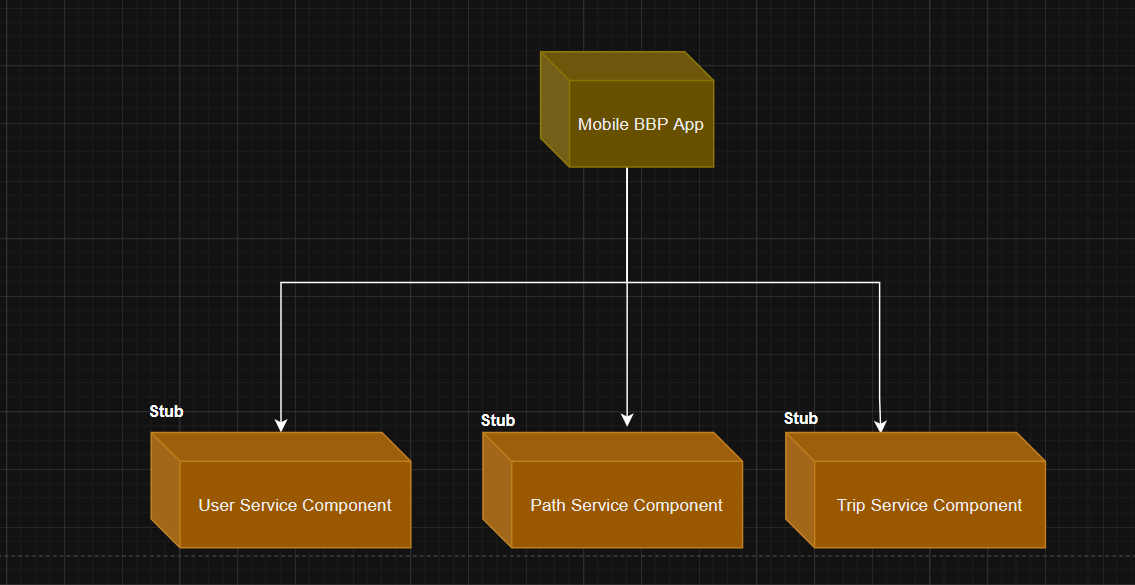
\includegraphics[width=0.5\linewidth]{DD/Images/Implementation/application.png}
    \caption{Testing BBP Mobile Application}
    \label{fig:placeholder}
\end{figure}




\begin{figure}[H]

    \centering
    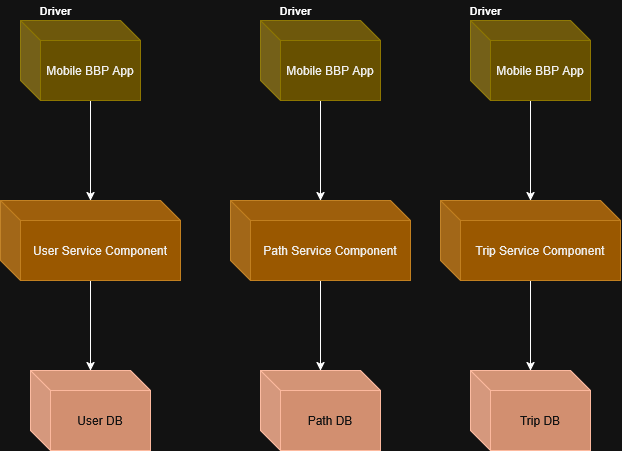
\includegraphics[width=0.5\linewidth]{DD/Images/Implementation/clusters.drawio.png}
    \caption{Unit Testing}
    \label{fig:placeholder}
\end{figure}


\begin{figure}[H]
    \centering
    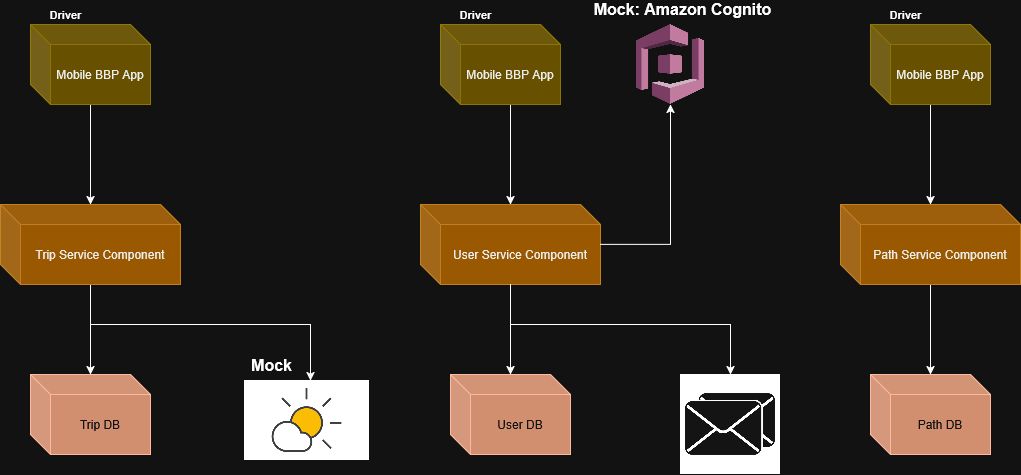
\includegraphics[width=0.5\linewidth]{DD/Images/Implementation/services.drawio.png}
    \caption{Mocking services in order to test each cluster}
    \label{fig:placeholder}
\end{figure}

\begin{figure}[H]
    \centering
    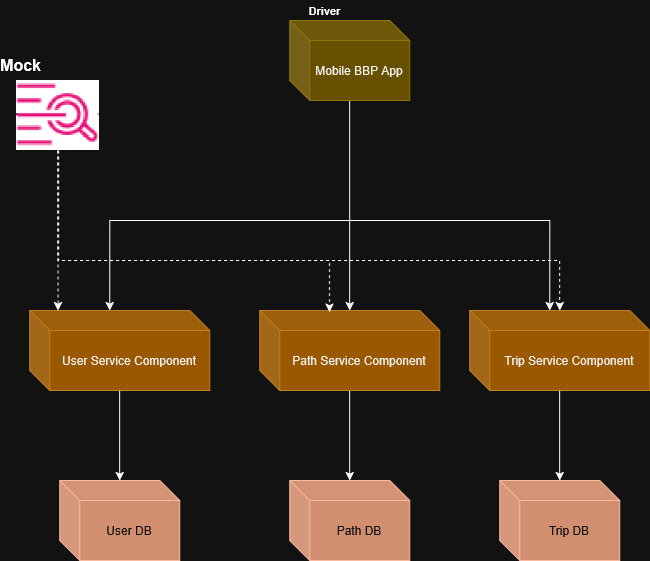
\includegraphics[width=0.5\linewidth]{DD/Images/Implementation/Discovery.drawio.png}
    \caption{Mocking Search and Discovery Service}
    \label{fig:placeholder}
\end{figure}
\begin{figure}[H]

    \centering
    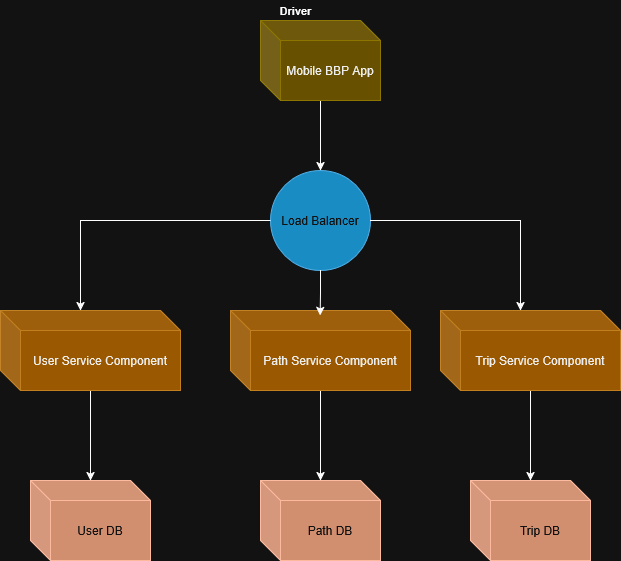
\includegraphics[width=0.5\linewidth]{DD/Images/Implementation/load.drawio.png}
    \caption{Testing at infrastructure level the load balancer}
    \label{fig:placeholder}
\end{figure}

